% Optional fragments; Markdown is the canonical V1. Captions retain evidence scope.
\begin{figure}[t]
\centering
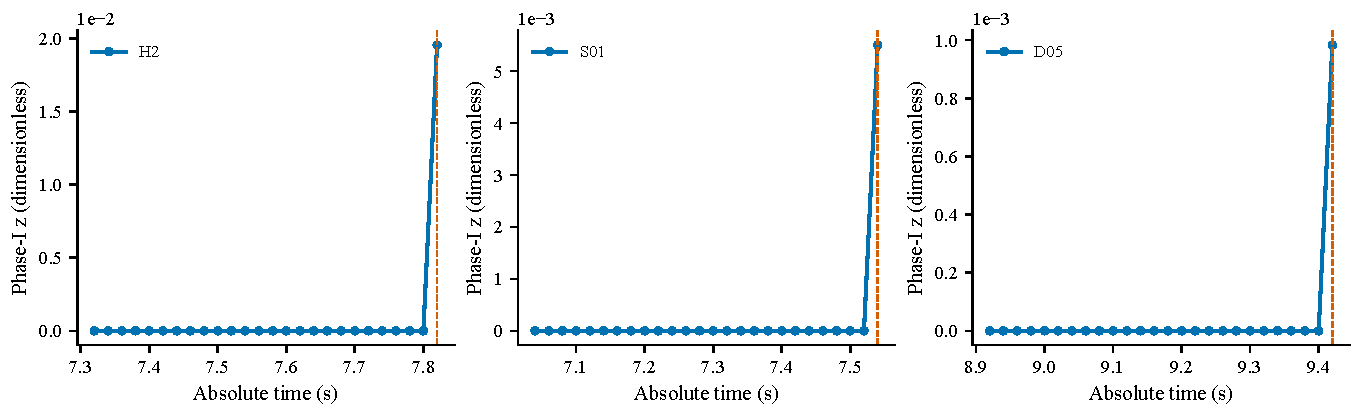
\includegraphics[width=0.95\textwidth]{figures/f1_historical_constraint_failure.pdf}
\caption{Historical H2, S01 and D05 frozen-set Phase-I analysis over the final0.5 s. Row scales are1 m/s for clearance and1 rad/s for joints. Dimensionless relaxation is not penetration or a feasible control. Dashed lines mark failed endpoints; no repaired trajectory is implied.}
\label{fig:historical-feasibility}
\end{figure}
\begin{figure}[t]
\centering
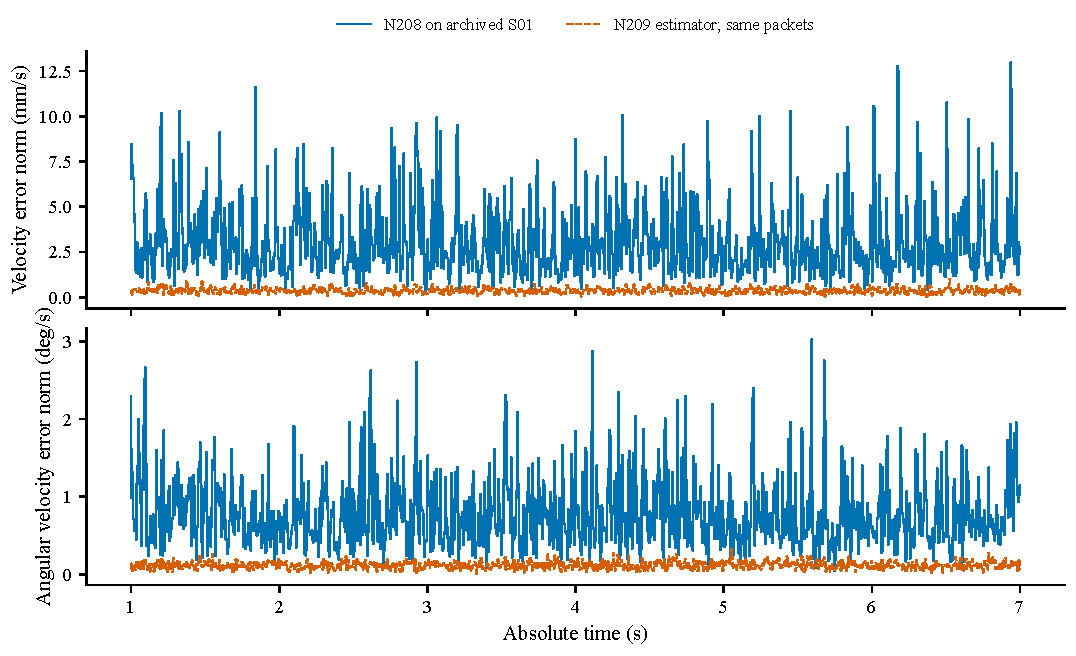
\includegraphics[width=0.95\textwidth]{figures/f2_same_packet_estimation.pdf}
\caption{Velocity error norms on identical archived S01 packets over absolute time1--7 s. Revised estimates are offline redecision outputs, not a new closed-loop capture. Error curves are not calibrated confidence bands.}
\label{fig:same-packet-estimator}
\end{figure}
\begin{figure}[t]
\centering
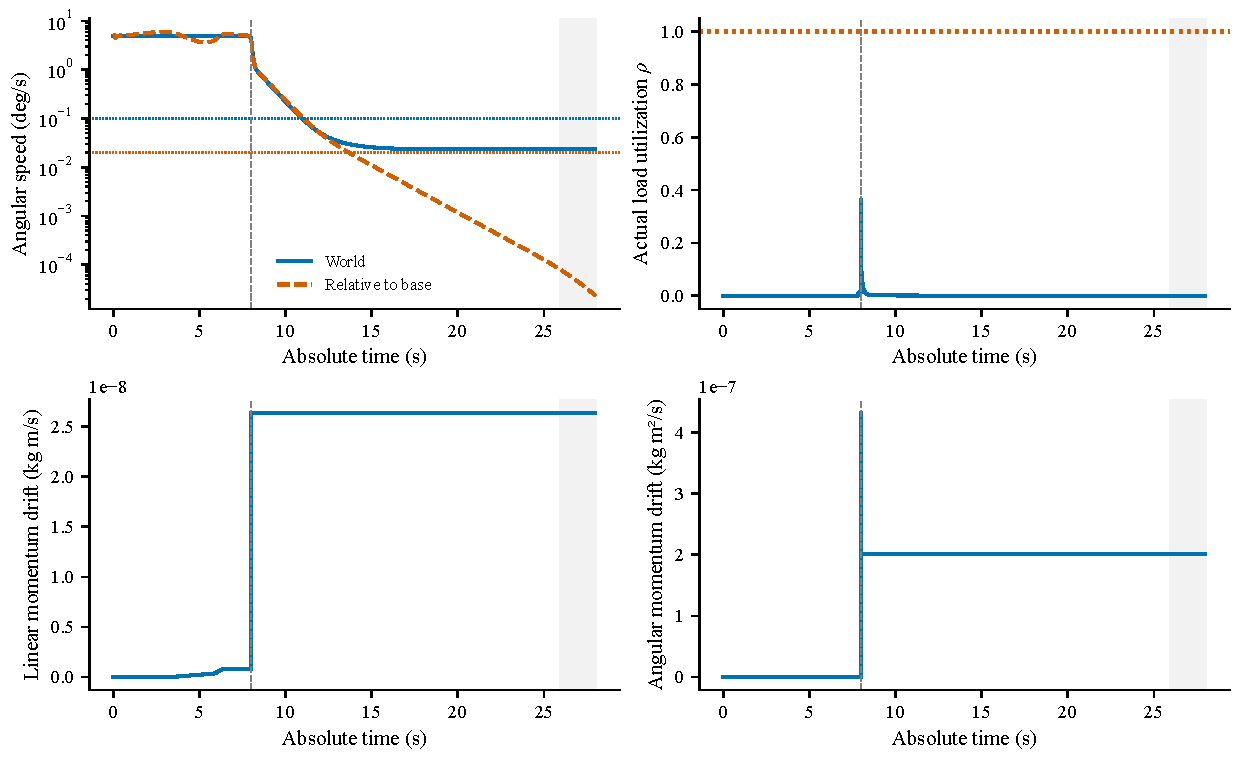
\includegraphics[width=0.95\textwidth]{figures/f3_nominal_continuous_task.pdf}
\caption{First nominal development run D01. Target world and target--base relative angular speed, actual load utilization, and separate total linear/angular momentum drift. Dashed line: latch at7.992 s. Shading: fixed final2 s,25.992--27.992 s. No numerical drift is removed from safety quantities; this is one seen scenario.}
\label{fig:nominal-continuous}
\end{figure}
\begin{figure}[t]
\centering
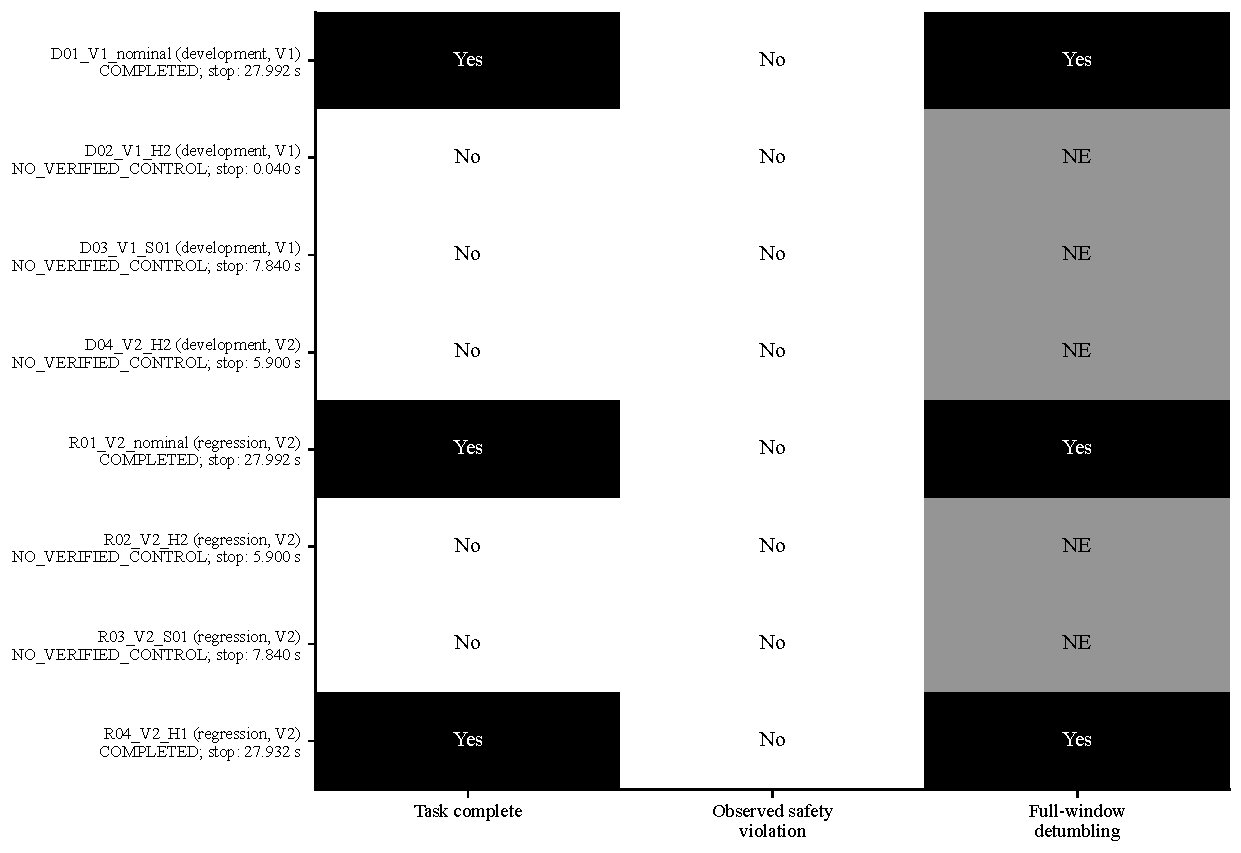
\includegraphics[width=0.95\textwidth]{figures/f4_all_attempt_outcomes.pdf}
\caption{All recorded N209 attempts, retaining category, version, status and stop time. Safety observations concern each recorded prefix. Gray NE means NOT\_EVALUATED, including unavailable full post-capture windows. Seen repetitions do not estimate independent success probability.}
\label{fig:all-attempts}
\end{figure}
\begin{figure}[t]
\centering
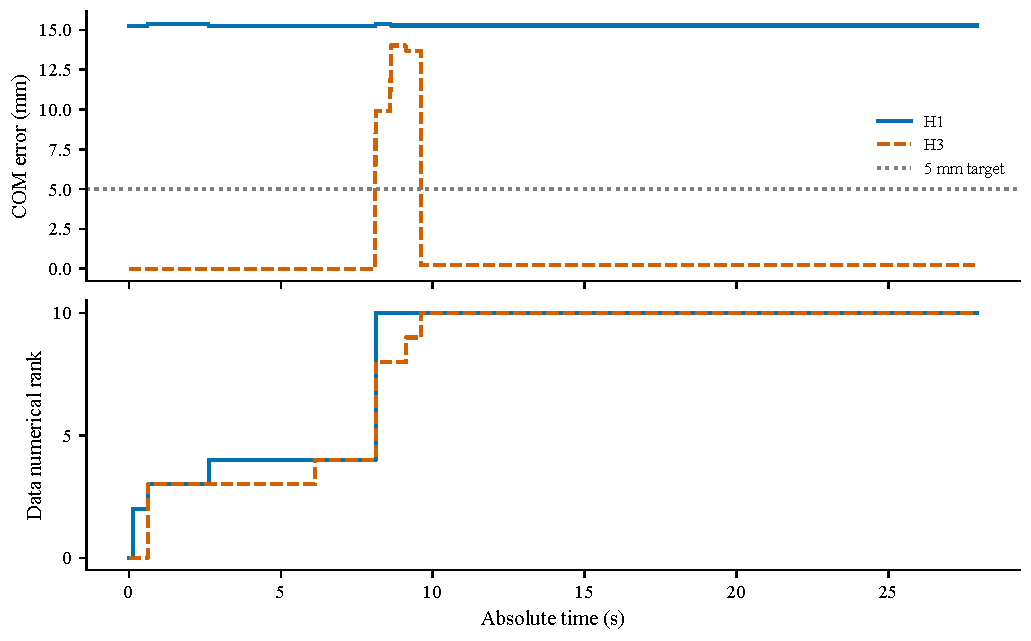
\includegraphics[width=0.95\textwidth]{figures/f5_historical_identification.pdf}
\caption{Historical H1 and H3 COM error and scaled whitened regressor rank. The5 mm COM target is unchanged. Rank ten does not ensure COM accuracy. Separate prior/identified paired trajectories have exactly zero maximum actuator difference in both scenarios despite posterior entry into prediction. Control benefit is not demonstrated.}
\label{fig:historical-identification}
\end{figure}
